\documentclass[11pt,a4paper,titlepage, ngerman]{article}

\usepackage[utf8]{inputenc}	% Diese Pakete sind
\usepackage[T1]{fontenc}		% für die Verwendung 
\usepackage{ngerman}			% von Umlauten im tex-file
\usepackage{lmodern}			% Schriftart, die am Bildschirm besser lesbar ist
\usepackage{graphicx}			% Zum Einbinden von Formeln
\usepackage{url}					% Zur Darstellung von Webadressen
\usepackage{siunitx}
\usepackage{amsmath}			% für equation*
\usepackage{subcaption}
\usepackage{wrapfig}

\begin{document}
%	\setlength{\parindent}{0em} 
	
	\begin{titlepage}
		\centering
		{\scshape\LARGE Versuchsbericht zu \par}
		\vspace{1cm}
		{\scshape\huge E4 -- Kennlinien\par}
		\vspace{2.5cm}
		{\LARGE Gruppe 10 Mi\par}
		\vspace{0.5cm}
		{\large Alex Oster (E-Mail: a\_oste16@uni--muenster.de) \par}
		{\large Jonathan Sigrist (E-Mail: j\_sigr01@uni--muenster.de ) \par}
		\vfill
		durchgeführt am 8.11.2017\par
		betreut von\par
		{\large David \textsc{Pahl}}
		
		\vfill
		
		{\large \today\par}
	\end{titlepage}
		
	\tableofcontents
	
	\newpage
	
	\section{Kurzfassung}
		
		In diesem Bericht befassen wir uns mit Kennlinien. Eine Kennlinie ist die Kurve, die entsteht, wenn man die Spannung gegen den Strom aufträgt. Aus dem Ohm'schen Gesetz $U=RI$ bzw. $I = \frac{1}{R}U $ ergibt sich, dass diese durch den Widerstand dargestellt wird. 
		
		Wir betrachten im Folgenden zwei Versuchen, die uns verschiedenen Arten von Widerständen näher bringen sollen. 
		
		In dem ersten Versuch betrachten wir fünf verschiedene Arten von Widerständen. Eine einfache Diode, eine Zenerdiode, einen NTC-Widerstand, eine Glüh- und eine Glimmlampe. Wir messen hierbei den Strom in Abhängigkeit von der Spannung und werten die Ergebnisse aus. Dazu gehen wir auf die Funktionsweise von Halbleitern und Glimmlampen ein. 
		
		Die Abhängigkeit des Widerstands von der Temperatur wird dann in dem zweiten Versuch betrachtet.
		Hierzu erhitzen wir einen Kupferdraht in Öl, lassen ihn danach abkühlen und messen durchgehend seinen Widerstand mit Hilfe einer Wheatstone'schen Brücke. Unsere Ergebnisse für den Kupferdraht verknüpfen wir dann mit der allgemeinen elektrischen Leitfähigkeit von Metallen.

	\section{Versuch 1: Strom-Spannungs-Charakteristik}
		
		\subsection{Methoden} %Aufbau und wie/was gemessen wird
		
		In Abb. \ref{Schaltskizze1} ist der Versuchsaufbau skizziert. Dabei fließt der Strom nur über jeweils einen Aufbau. 
		
		Da die Spannungsquelle keine genaue Angabe der Eingangsspannung liefert, messen wir diese mit einem Multimeter, welches parallel zu dem Aufbau geschaltet ist. Den Strom hingegen messen wir mit einem zweiten Multimeter, welches in Reihe zu dem Aufbau geschaltet ist.
		
		Für die Teilversuche a) bis d) verwenden wir Eingangsspannungen im Bereich von \SIrange{0}{20}{\V} und für die Glimmlampe in e) Eingangsspannungen von \SIrange{0}{150}{\V}.
		
		\begin{figure}
			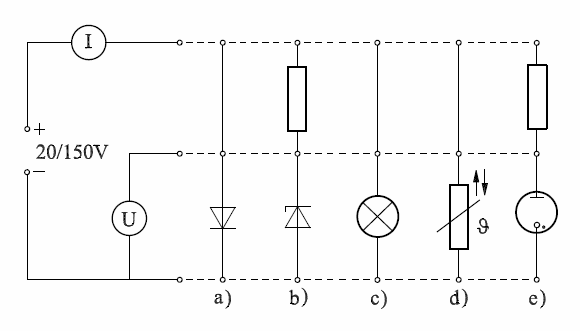
\includegraphics[width=\textwidth]{Versuch1.png}
			\caption{Schaltskizze zu Versuch 1}
			\label{Schaltskizze1}
		\end{figure}

		\subsection{a) Diode in Durchlassrichtung} 
			
			\subsubsection{Diode}
			
				Eine Diode ist ein Bauteil, mit dem Spannungen nur von einer Richtung durchgelassen werden. Diesen Effekt erhält man, wenn man einen Halbleiter mit einem Element aus der dritten Hauptgruppe dotiert (p-Leiter) und einen anderen mit einem Element aus der fünften Hauptgruppe (n-Leiter) und diese aneinander grenzen lässt. Hierbei entsteht eine Raumladungszone im Übergangsbereich, da die Elektronen des n-Leiters zu dem p-Leiter wandern. Da in dem Übergangsbereich weniger freie Ladungsträger sind, als im restlichen Leiter, nimmt die Leitfähigkeit an dieser Stelle stark ab.
				
				Legt man den positiven Pol einer aüßeren Spannung an den n-Leiter an, so vergrößert sich der Übergangsbereich. Bei einem negativen Pol hingegen, verkleinert sich dieser, sodass der Strom durch den Leiter fließen kann. 
			
			\subsubsection{Messung}
				
				Wie in Abb. \ref{} zu sehen ist, verläuft die Kennlinie bei einer Diode in Durchflussrichtung %TODO
			
			\subsubsection{Schlussfolgerung}
			
				Unsere Ergebnisse deuten darauf hin, dass %TODO
				
		\subsection{b) Zenerdiode} %Erklärung Zenerdioden, Messung und Schlussfolgerung
			
			Die Zenerdiode
			
			\subsubsection{in Sperrrichtung}
			
			\subsubsection{in Durchlassrichtung}
			
		\subsection{c) Glühlampe} %Erklärung Glühlampe als Widerstand, Messung und Schlussfolgerung

		\subsection{d) NTC-Widerstand} %Erklärung NTC, Messung und Schlussfolgerung

		\subsection{e) Glimmlampe} %Erklärung Glimmlampe, Messung und Schlussfolgerung

	\section{Versuch 2: Widerstand in Abhängigkeit der Temperatur}		

		\subsection{Methoden} %Aufbau und wie/was gemessen wird
		
		\subsection{Messung}
		
		\subsection{Schlussfolgerung}		
	
	\newpage	
	\begin{thebibliography}	
		e empty
	\end{thebibliography}	
			
\end{document} 